\documentclass{bioinfo}
\copyrightyear{2014}
\pubyear{2014}

\begin{document}
\firstpage{1}

\title[DNAplotlib]{DNAplotlib: standardized visualization of genetic constructs, libraries and associated data}
\author[Thomas E. Gorochowski \textit{et~al.}]{Thomas~E.~Gorochowski$^{1}$, Bryan~Der$^{1}$, Emerson~Glassey$^{1}$, D. Benjamin Gordon$^{1}$ and Christopher~A.~Voigt$^{1,}$\footnote{to whom correspondence should be addressed}}
\address{$^{1}$Department of Biological Engineering, Synthetic Biology Center, Massachusetts Institute of Technology, USA.}

\history{Received on XXXXX; revised on XXXXX; accepted on XXXXX}

\editor{Associate Editor: XXXXXXX}

\maketitle

\begin{abstract}

\section{Summary:}
DNAplotlib is a computational toolkit that enables highly customizable visualization of single genetic constructs and libraries of design variants. Publication quality vector-based output is produced and all aspects of the rendering process can be easily customized or extended by the user. DNAplotlib is capable of outputting SBOL Visual compliant diagrams, in addition to a trace-based format that is able to better illustrate the precise location and length of each genetic part. This alternative visualization method enables direct comparison with nucleotide-level data such as RNA-seq read depth. While it is envisaged that access will be predominantly via the programming interface, command-line and web-based front-ends are also provided to support broader usage.

\section{Availability:}
DNAplotlib is cross-platform and open-source software developed using Python and released under the OSI recognized NPOSL-3.0 license. Source code, documentation and a web front-end are available at the project website: \href{http://www.dnaplotlib.org}{http://www.dnaplotlib.org}.

\section{Contact:} \href{cavoigt@gmail.com}{cavoigt@gmail.com}
\end{abstract}

Engineering disciplines rely on standardized pictorial representations of parts and their interconnections to clearly communicate how these should be pieced together and allow for the reliable construction of large complex systems. In biology, DNA sequences are often engineered to create genetic constructs that probe or perturb the function of natural systems, or more recently, create novel capabilities in what has been termed ``synthetic biology'' \citep{Church14a}. Unlike traditional engineering fields, the way that these genetic designs are visually represented varies significantly between labs and across different areas of the field. This leads to ambiguities that can hinder understanding and the effective reuse of research. The Synthetic Biology Open Language (SBOL) Visual initiative was started to help alleviate this problem by defining a set of agreed symbols for commonly used genetic elements \citep{Quinn13a}, see Fig.~\ref{fig:overview}A. However, so far this standard has seen limited uptake due to a lack of accessible tools that can be directly integrated into existing design and analysis workflows.

To our knowledge, the only attempt so far to automate the creation of standard-compliant diagrams has been PigeonCAD \citep{Bhatia13a}. This web-based tool interprets a custom syntax used to specify genetic designs and automatically transforms these into visual representations. The main issues with this tool are: (i)~it does not provide access to the full set of SBOL symbols limiting the types of construct it can display, (ii)~output is in the form of poor-quality images that do not scale well, and (iii)~the fixed design syntax restricts the ability for users to customize visualizations for their specific needs or extend the functionality to include new forms of part. Furthermore, synthetic biology is increasingly pushing towards automated design procedures that harness the potential to construct huge libraries of design variants \citep{Smanski14a,Bilitchenko11a}, see Fig.~\ref{fig:overview}D. Under these scenarios, efficient automation of visualization tasks is essential to ensure clear communication of these large design spaces. The inability to tightly integrate PigeonCAD into such workflows makes it unsuitable for these tasks.

\begin{figure}[tb]
\centering
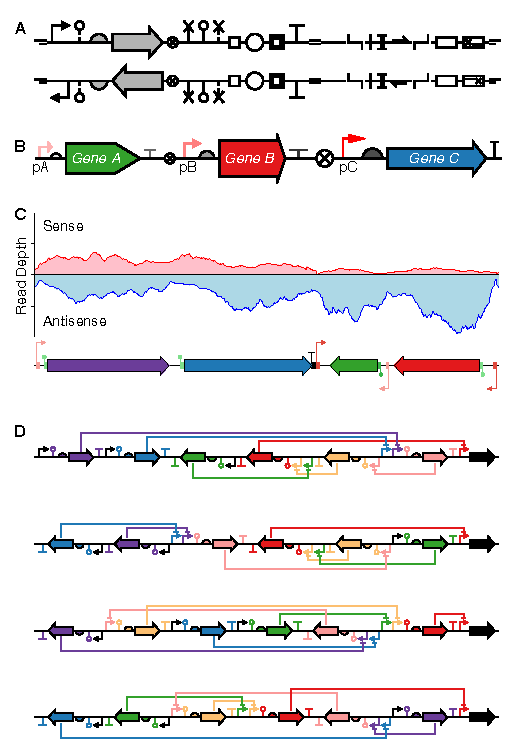
\includegraphics[width=8.3cm]{Figure1.pdf}
\caption{\label{fig:overview}Overview of core DNAplotlib functionality. All visualizations were generated driectly from DNAplotlib. (\textbf{A})~The complete set of SBOL Visual parts that capture the majority of widely used genetic elements are available for use in both forward and reverse orientations. (\textbf{B})~The size, color, shape and labeling of all elements can be easily customized enabling additional information to be communicated e.g., promoter strengths or spacer lengths. Users can further supply their own functions to draw parts in a non-standard way or to represent new types of genetic element yet to be incorporated into SBOL Visual. (\textbf{C})~To facilitate direct comparison between a genetic design and associated nucleotide-level data, such as RNA-seq read depths, trace-based renderers are also provided. These use the standard promoter and terminator symbols and a small filled circle to represent an RBS. Indicators of actual part widths (arrow length for coding sequences and small filled rectangles for promoters and RBSs) are displayed on the DNA backbone to enable a clear visual alignment of design information with trace data. (\textbf{D})~Visualization of a library of genetic design variants implementing the same 3-input (black promoters), 1-output (black coding sequences) device. Colors have been used to link repressor genes to their cognate promoters.}
\end{figure}

To address these limitation we developed a computational toolkit called DNAplotlib that enables highly-customizable visualization of genetic constructs in a programmable way (Fig.~\ref{fig:overview}B). DNAplotlib has been developed in Python and makes significant use of matplotlib \citep{Hunter07a}, a 2D graphics library that can produce graphical output in the form of vector-based PDFs or rasterized images e.g., JPEGs. Python was chosen as the underlying language due to its increasing use in the analysis of biological data \citep{Cock09a}, which enables visualizations generated by DNAplotlib to be integrated into existing analysis workflows with minimal effort. Furthermore, Python is highly-portable ensuring availability of our tools across all major operating systems.

At the core of the toolkit is the main rendering pipeline. This is structured such that individual functions are provided when run to draw each symbol type. Standard built-in functions can be chosen that cover the full range of SBOL Visual parts (Fig.~\ref{fig:overview}A), or the user can specify their own which may include new forms of part type not currently available. In addition, we also provide what are termed trace-based renderers that draw promoters, ribosome binding sites (RBSs), coding sequences (CDSs) and terminators such that the start and end points relate to their actual position within a construct (Fig.~\ref{fig:overview}C). Unlike the conceptual SBOL Visual renderers where only ordering and orientation information are maintained, trace-based renders allow for a direct comparison between nucleotide-level data and the associated design information, see Fig.~\ref{fig:overview}C.

To create a visualization, designs are provided in the form of a standard list data type, where each element is a dictionary defining the part at that position and any other design information, e.g., orientation, length and styling options. By using a dictionary, varying options for each part type can be easily accommodated. Visualizations are then generated by scanning this list and calling functions associated to each part type encountered. If a part type is unknown or an attribute not used, this element is ignored ensuring that renderers providing differing levels of functionality do not break the entire pipeline. Regulation is handled in a similar way with start and end points provided in addition to styling options. All rendering is performed using a matplotlib axis, allowing for genetic designs to be incorporated into standard plotting routines.

Although directly accessing DNAplotlib from Python gives greatest flexibility, in many cases it is simpler for a user to specify designs and part customizations in text-based files. These can be shared more easily and allow for better reuse of design or styling information. For these purposes we developed two command-line interfaces. The first mimics the idea of PigeonCAD using a simple syntax to define basic constructs as a single line of text. This is useful for the quick creation of small constructs with limited customization. The second is designed for visualization of large libraries of designs. Users are required to provide several text files defining the parts, their styling, and the part ordering, orientation and regulatory links. These are then processed and a visualization of the full library output.

To further ensure broadest access to non-programmers, web-based interfaces for each of these command-line scripts is available. These were developed using Jetty and provide a graphical user interface for creating simple constructs and the ability to upload text-based files of library designs. Visualizations can be previewed and downloaded as JPEG or PDF files.

DNAplotlib is under continual development with a current focus on broadening the types of genetic element covered to include new synthetic biological parts. The project welcomes contributions from others within the community through the project website and public development repository: \href{http://www.dnaplotlib.org}{http://www.dnaplotlib.org}.

\section*{ACKNOWLEDGEMENTS}
T.E.G., B.D., E.G., D.B.G. and C.A.V. were supported by...

\begin{thebibliography}{}
\bibitem[Church {\it et~al}., 2014]{Church14a} Church, G.M., Elowitz, M.B., Smolke, C.D., Voigt, C.A. and Weiss, R. (2014). Realizing the potential of synthetic biology, {\it Nat. Rev. Mol. Cell Biol.}, {\bf 15}, 289-294.

\bibitem[Bhatia \& Densmore, 2013]{Bhatia13a} Bhatia, S. and Densmore, D. (2013). Pigeon: A Design Visualizer for Synthetic Biology, {\it ACS Synth. Biol.}, {\bf 2}, 348-350.

\bibitem[Smanski {\it et~al}., 2014]{Smanski14a} Smanski, M.J., Swapnil, B., Park, YJ., Zhao, D., Giannoukos, G., Ciulla, D., Busby, M., Calderon, J., Nicol, R., Gordon, D.B., Densmore, D. and Voigt, C.A. (2014) Combinatorial design and assembly of refactored gene clusters, {\it Nat. Biotech.}, {\bf ?}, ???-???.

\bibitem[Hunter, 2007]{Hunter07a} Hunter, J.D. (2007). Matplotlib: A 2D graphics environment, {\it Computing in Science \& Engineering}, {\bf 9}, 90-95.

\bibitem[Cock {\it et~al}., 2009]{Cock09a} 
Cock PJ, Antao T, Chang JT, Chapman BA, Cox CJ, Dalke A, Friedberg I, Hamelryck T, Kauff F, Wilczynski B, and de Hoon MJ. (2009) Biopython: freely available Python tools for computational molecular biology and bioinformatics. {\it Bioinformatics}, {\bf 25}, 1422-1422.

\bibitem[Bilitchenko {\it et~al}., 2011]{Bilitchenko11a} 
Bilitchenko, L., Liu, A., Cheung, S., Weeding, E., Xia, B., Leguia, M., Anderson, J.C., Densmore, D. (2011) Eugene – A Domain Specific Language for Specifying and Constraining Synthetic Biological Parts, Devices, and Systems. {\it PLoS ONE}, {\bf 6}, e18882.

\bibitem[Quinn {\it et~al}., 2013]{Quinn13a} 
Quinn, J., Beal, J., Bhatia, S., Cai, P., Chen, J., Clancy, K., Hillson, N., Galdzicki, M., Maheshwari, A.P., Umesh; P., Matthew; R.C.; Stan, G.-B., Endy, D. (2013) ``Synthetic Biology Open Language Visual (SBOL Visual), version 1.0.0.''

\end{thebibliography}

\end{document}
